\documentclass[10pt]{beamer}
\usetheme[
%%% option passed to the outer theme
%    progressstyle=fixedCircCnt,   % fixedCircCnt, movingCircCnt (moving is deault)
  ]{Feather}
  
% If you want to change the colors of the various elements in the theme, edit and uncomment the following lines

% Change the bar colors:
%\setbeamercolor{Feather}{fg=red!20,bg=red}

% Change the color of the structural elements:
%\setbeamercolor{structure}{fg=red}

% Change the frame title text color:
%\setbeamercolor{frametitle}{fg=blue}

% Change the normal text color background:
%\setbeamercolor{normal text}{fg=black,bg=gray!10}

%-------------------------------------------------------
% INCLUDE PACKAGES
%-------------------------------------------------------

\usepackage[utf8]{inputenc}
\usepackage[english]{babel}
\usepackage[T1]{fontenc}
\usepackage{helvet}

%-------------------------------------------------------
% DEFFINING AND REDEFINING COMMANDS
%-------------------------------------------------------

% colored hyperlinks
\newcommand{\chref}[2]{
  \href{#1}{{\usebeamercolor[bg]{Feather}#2}}
}

%-------------------------------------------------------
% INFORMATION IN THE TITLE PAGE
%-------------------------------------------------------

\title[] % [] is optional - is placed on the bottom of the sidebar on every slide
{ % is placed on the title page
      \textbf{Flood prediction using Machine Learning}
}

\subtitle{e-Yantra Ideas Competition 2019-20}


\author{Varad Kshemkalyani \\* Heer Kukreja \\* Pratheek Menon \\* Reuben Thomas}

\institute[]
{
    Vivekanand Institute Of Technology, Chembur\\
  %there must be an empty line above this line - otherwise some unwanted space is added between the university and the country (I do not know why;( )
}

%-------------------------------------------------------
% THE BODY OF THE PRESENTATION
%-------------------------------------------------------

\begin{document}

%-------------------------------------------------------
% THE TITLEPAGE
%-------------------------------------------------------

{\1% % this is the name of the PDF file for the background
\begin{frame}[plain,noframenumbering] % the plain option removes the header from the title page, noframenumbering removes the numbering of this frame only
  \titlepage % call the title page information from above
\end{frame}}


\begin{frame}{Table of Contents}{}
\tableofcontents
\end{frame}

%-------------------------------------------------------
\section{Introduction/Motivation}
%-------------------------------------------------------

\begin{frame}{Introduction/Motivation}
%-------------------------------------------------------

  \begin{itemize}
    \item The degree and scale of flood hazards have increased massively with the changing climate in the last decades, resulting in tremendous life and property losses as well as social disruption worldwide. Cutting of mangroves and trees in coastal regions and river plains for land development has led to decreasing water retention and increasing surface runoff which in turn increases the probability of flash floods. Thus, flood prediction and flood control are important issues for policy makers and designers.
    \end{itemize}
\end{frame}
\begin{frame}{Introduction/Motivation}
    \begin{itemize}
    \item To mimic the complex mathematical expressions of physical processes of floods, during the past two decades, machine learning (ML) methods and Artificial intelligence (AI) contributed highly in the advancement of prediction systems providing better performance and cost-effective solutions.
   \end{itemize}
\end{frame}
\begin{frame}{Introduction/Motivation}
\begin{itemize} 
 \item Flooding depends on factors such as rainfall, elevation, bank heights, drainage distance, soil properties and land use. Our proposed system will identify food prone regions and link flooding to deforestation in the area to allow sustainable growth in the future by giving afforestation as a solution to mitigate effects of floods.
  \end{itemize}
\end{frame}

%-------------------------------------------------------
\section{Market Research / Literature Survey}
%-------------------------------------------------------
\subsection{Market Research}
\begin{frame}{Market Research}
%-------------------------------------------------------
\end{frame}

%-------------------------------------------------------
\subsection{}
\begin{frame}{Market Research}
%-------------------------------------------------------

\end{frame}
    

%-------------------------------------------------------
\section{Requirements}
\subsection{Software and Hardware Requirements}

%-------------------------------------------------------
\begin{frame}{Requirements}{Software and Hardware Requirements}
  \begin{block}{Software Requirements}
  \begin{itemize}
    \item {\tt Scikit-Learn} \vspace{5pt}
    \item {\tt Tensorflow} \vspace{5pt} 
    \item {\tt Azure Machine Learning Lab} \vspace{5pt} 
    \item {\tt Keras.io} \vspace{5pt} 
    \item {\tt ArcGIS Online} \vspace{5pt} 
    \end{itemize}  
  \end{block}
\end{frame}


%-------------------------------------------------------
\section{Implementation}
%-------------------------------------------------------
\subsection{}
\begin{frame}{Implementation}

%-------------------------------------------------------

\begin{block}{}
    \begin{itemize}
    \item Our project aims at predicting floods in various susceptible areas along water bodies. The risk of flooding is increasing as a result of deforestation, untimely and torrential rains, sea level rise, concretization and unscentific developement etc. 
    \item To avoid devastating consequences which have a major impact on economic and financial conditions of the city, our system aims to provide maximum accuracy in alerting target regions about the forthcoming disasters.
    \item This model can be extended for different locations in the future.
       
    \end{itemize} 
\end{block}
\end{frame}

\begin{frame}{Implementation}{Using GIS}
\begin{block}{}
\begin{itemize}
\item \small Flood-influencing factors as independent variables are essential to generate a flood susceptibility map . \item Scarcity of data can limit the the number of models that can be used to identify flood risk zones. A possible solution to this can be the use of GIS (Geographical Information System) based models to provide a more accurate prediction.\item  GIS coupled with various models have been used before to create flood susceptibility maps.\item Analysing the factors afecting the floods using the learning vector quantization process(LVQ) will help us identify the major contributing factor. We will use statistical data based on various factors, maps and images. \item The datasets can either be real-time data collected from Synthetic Aperture Radar(SAR) or historical data recorded before.
\end{itemize} 
\end{block}
\end{frame}

\begin{frame}{Implementation}
    \begin{block}{}
            \begin{figure}
	            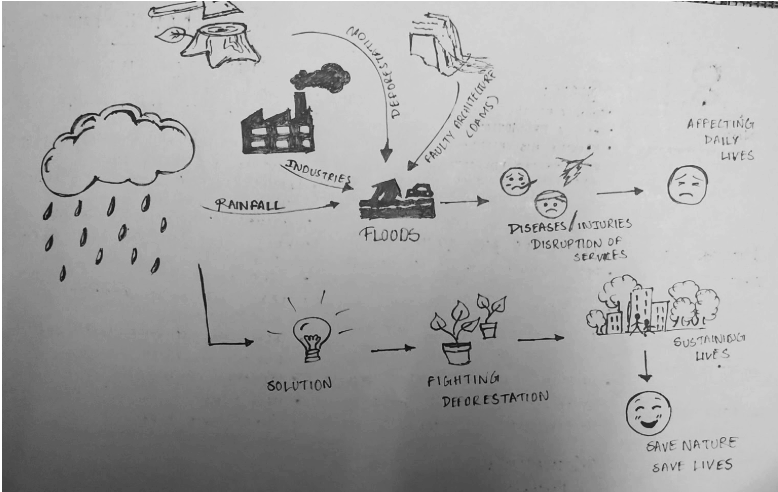
\includegraphics[width=100mm,height=55mm]{journeymap.png}
	            {\tt Journey Map from adverse effects of floods \& deforestation to a greener and sustainable future.}
	            \label{fig:map}
            \end{figure}
    \end{block}
\end{frame}


\begin{frame}{Feasibility}
    \begin{block}{}
        \begin{itemize}
            \item The risk of coastal flooding is increasing as a result of deforestation, untimely and torrential rains, sea level rise etc. In the event of floods occurring, a large amount of damage can be curbed if we have a model that could predict floods in advance. 
            \item Not many ways we use today for addressing environmental challenges employ evolving and proven technologies like Artificial Intelligence and Machine Learning visible in inaccurate results (e.g. erroneous weather predictions etc). 

         \end{itemize}
    \end{block}
\end{frame}



%-------------------------------------------------------
\section{Feasibility}
%-------------------------------------------------------
\subsection{}
\begin{frame}{Feasibility}
    \begin{block}{}
        \begin{itemize}
            \item The methods which are currently being used to address floods and other environmental challenges have a high degree of uncertainty associated with them.
            \item With a reliable flood prediction model in place, government authorities in the targeted regions will be alerted about the impending floods in advance and will hence be able to evacuate the people living there and minimize other damages caused by the floods.
         \end{itemize}
    \end{block}
\end{frame}


{\1
\begin{frame}[plain,noframenumbering]
  \finalpage{\LARGE \textbf{\emph{Thank You!}}}
\end{frame}}

\end{document}